\subsection{VQ-VAE}
\begin{frame}{}
	\LARGE VAE: \textbf{Vector Quantized VAE (VQ-VAE)}
\end{frame}

\begin{frame}{VQ-VAE: Discrete Latent Codes}
\begin{itemize}
    \item \textbf{VQ-VAE} (van den Oord et al., 2017) replaces the Gaussian latent with a \textbf{codebook}: $K$ learnable embedding vectors $e_1, \ldots, e_K$ (e.g.\ $K = 512$).
    \item The encoder produces a \textbf{grid} of vectors, and each one is \textbf{snapped to its nearest codebook entry}; an image becomes a small grid of discrete token indices (e.g.\ $32 \times 32$ for ImageNet).
    \item Why discrete?
    \begin{itemize}
        \item Much of the world is naturally discrete: words, phonemes, object identities.
        \item A code must commit to \textbf{one} codebook entry; there is no Gaussian averaging between concepts.
        \item With a uniform prior over codes, the KL term is a \textbf{constant}: no reconstruction-vs-KL balancing act and no posterior collapse.
    \end{itemize}
\end{itemize}
\end{frame}

\begin{frame}[allowframebreaks]{VQ-VAE: Architecture}
\begin{figure}
        \centering
        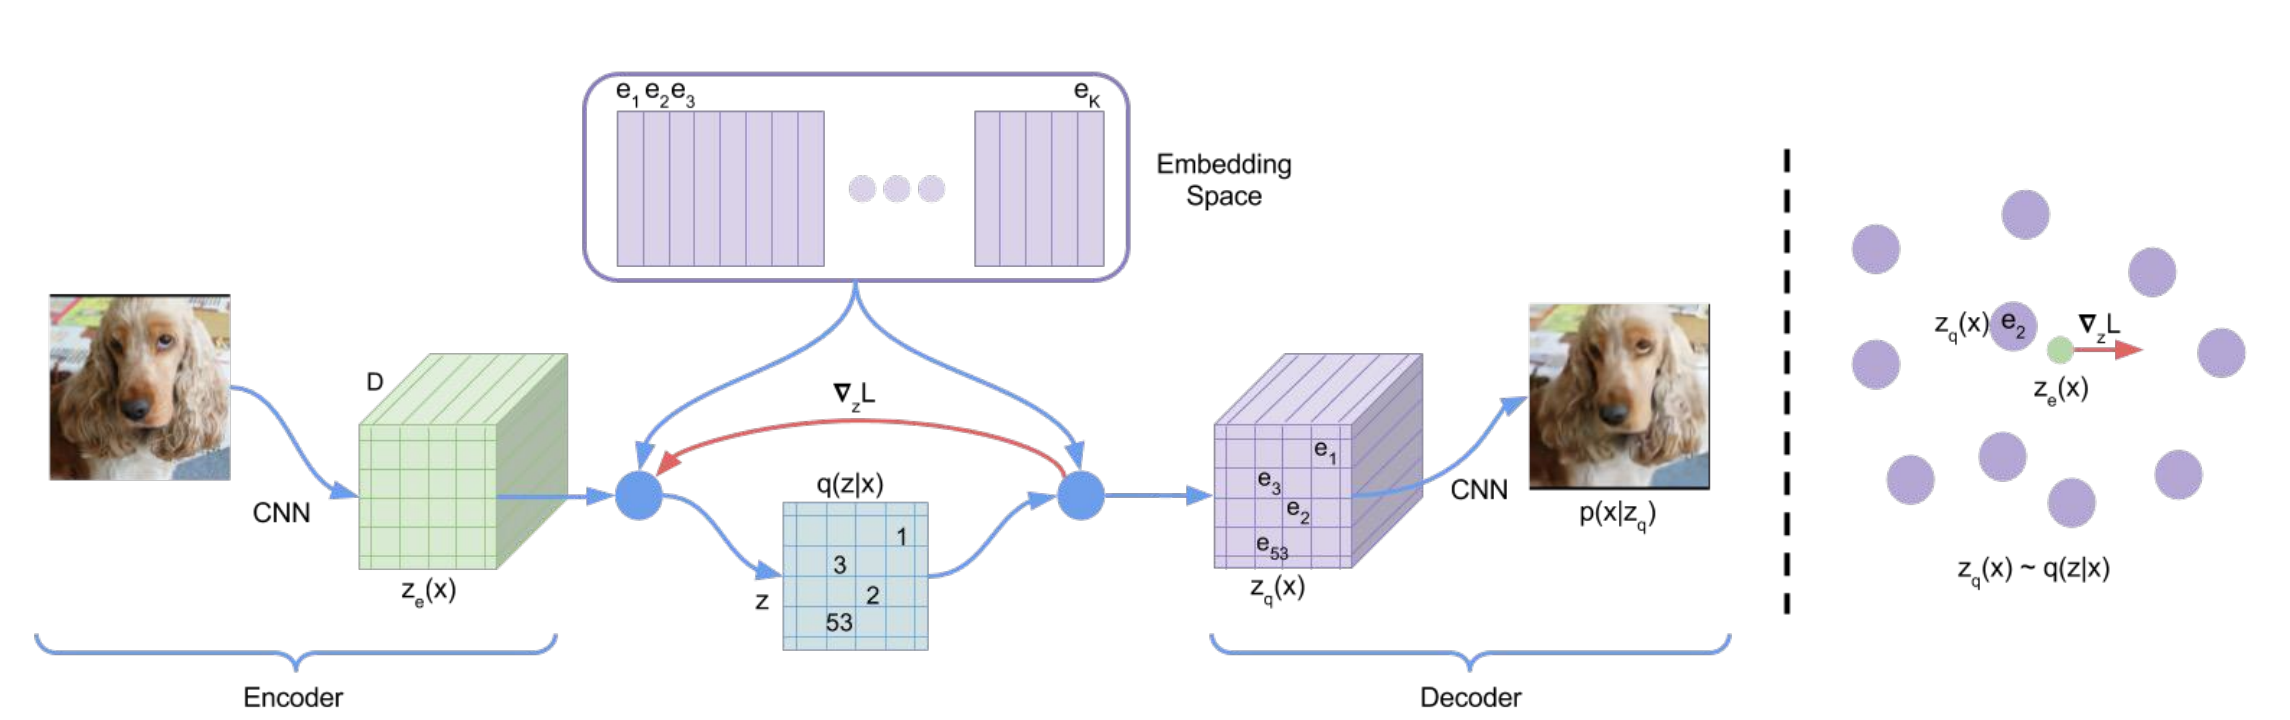
\includegraphics[height=0.8\textheight, width=\textwidth, keepaspectratio]{images/vae/vqvae.png}
        \caption*{\scriptsize Source: van den Oord, Vinyals \& Kavukcuoglu, ``Neural Discrete Representation Learning,'' NeurIPS 2017, Fig.~1.}
\end{figure}
\end{frame}

\begin{frame}[allowframebreaks]{VQ-VAE: Discrete Posterior}

\begin{itemize}
    \item A latent embedding space $e \in \mathbb{R}^{K \times D}$ where $K$ is the size of the discrete latent space ($K$-way categorical distribution)
    \item  Encoder output $z_e(x)$ is mapped to discrete latent code $z$ by a nearest neighbour look-up using the shared embedding space $e$
    \item The posterior categorical distribution $q(z|x)$ probabilities are defined as one-hot as:
    \[ q(z = k|x) = \begin{cases}
          1 & \text{for } k = \operatorname*{arg\,min}_j \|z_e(x) - e_j\|_2 \\
          0 & \text{otherwise}
       \end{cases}
    \]
\end{itemize}
\end{frame}

\begin{frame}[allowframebreaks]{VQ-VAE: Quantization and Loss}
\begin{itemize}
    \item  This model can be seen as a VAE in which the proposal distribution $q(z = k|x)$ is deterministic.
    \item The representation $z_e(x)$ is passed through the discretization bottleneck followed by mapping onto the nearest element of embedding $e$\\
    \[ z_q(x) = e_k, \hspace{1cm} \text{where} \hspace{0.5cm} k = \operatorname*{arg\,min}_j \|z_e(x) - e_j\|_2 \]
    \[ \mathcal{L} = -\log p(x \mid z_q(x)) + \|\mathrm{sg}[z_e(x)] - e\|^2_2 + \beta \|z_e(x) - \mathrm{sg}[e]\|_2^2 \]
    sg stands for the \textbf{stopgradient} operator that is defined as identity at forward computation time and has zero partial derivatives, thus effectively constraining its operand to be a non-updated constant.
    \item The embedding space is learned via Vector Quantization (VQ), whose objective uses the $l_2$ error to move the embedding vectors $e_i$ towards the encoder outputs $z_e(x)$

\end{itemize}
\end{frame}

\begin{frame}{The Gradient Problem: arg\,min Is Not Differentiable}
\begin{itemize}
    \item Picking the nearest codebook entry is a \textbf{hard selection}: the mapping $z_e \mapsto z_q$ is piecewise constant, so its gradient is \textbf{zero almost everywhere} (and undefined on the boundaries).
    \item Backpropagation from the decoder therefore stops dead at the quantization step; the encoder would never learn.
    \item \textbf{Straight-through estimator:} in the forward pass use $z_q$; in the backward pass \textbf{copy the gradient} $\nabla_{z_q} \mathcal{L}$ straight to $z_e$, as if quantization were the identity.
    \item This is an approximation, but a reasonable one because the commitment loss keeps $z_e$ close to the codebook entry it maps to.
    \item Same family of tricks as the discrete VAE's Gumbel-Softmax from the variants slide; VQ-VAE's version is simpler and works at scale.
\end{itemize}
\end{frame}

\begin{frame}{The Three Terms of the VQ-VAE Loss}
\[
\mathcal{L} \;=\; \underbrace{-\log p(x \mid z_q(x))}_{\text{1. reconstruction}} \;+\; \underbrace{\|\mathrm{sg}[z_e(x)] - e\|_2^2}_{\text{2. codebook loss}} \;+\; \underbrace{\beta \, \|z_e(x) - \mathrm{sg}[e]\|_2^2}_{\text{3. commitment loss}}
\]
\begin{itemize}
    \item \textbf{1. Reconstruction:} trains the \textbf{decoder} directly and the \textbf{encoder} through the straight-through gradient copy.
    \item \textbf{2. Codebook loss:} the stop-gradient freezes the encoder output, so only the \textbf{codebook entries} move toward their assigned encoder outputs (EMA updates are an alternative).
    \item \textbf{3. Commitment loss:} the stop-gradient freezes the codebook, so only the \textbf{encoder} moves; it commits to its entry instead of drifting; $\beta \approx 0.25$.
    \item Each term has one job; the two stop-gradients keep the jobs separate.
\end{itemize}
\end{frame}

\begin{frame}{Two-Stage Training: Codebook First, Prior Second}
\begin{itemize}
    \item \textbf{Stage 1} trains encoder, decoder, and codebook with the loss above. The prior over codes is assumed \textbf{uniform}, so the KL term is constant and simply dropped.
    \item But sampling a uniformly random grid of tokens decodes to noise: real images use \textbf{structured} combinations of codes.
    \item \textbf{Stage 2:} freeze everything from stage 1 and fit an \textbf{autoregressive prior} over the discrete code grid: PixelCNN for images, WaveNet for audio. To generate: sample a code grid from the prior, then decode it.
    \item \textbf{Why two stages?} It separates \textbf{perceptual compression} (stage 1) from \textbf{distribution modeling} (stage 2), and the prior works on a small token grid ($32 \times 32$) instead of $128^2$ pixels.
    \item This blueprint outlived VQ-VAE: VQ-VAE-2, VQGAN with transformers, DALL·E 1, and the tokenizer-plus-generator pattern of modern latent generative models all follow it.
\end{itemize}
\end{frame}

\begin{frame}{VQ-VAE}
    \begin{columns}
\begin{column}{0.4\textwidth}
   \begin{itemize}
       \item For speech, images, and videos one can extract 1D, 2D, and 3D latent feature spaces respectively
       \item  $32 \times 32$ latents for ImageNet, or $8 \times 8 \times 10$ for CIFAR10
       \item 1D sequences of latents drawn from a 512-entry codebook ($K=512$) for VCTK and LibriSpeech
   \end{itemize}
\end{column}
\begin{column}{0.6\textwidth}
    \begin{center}
     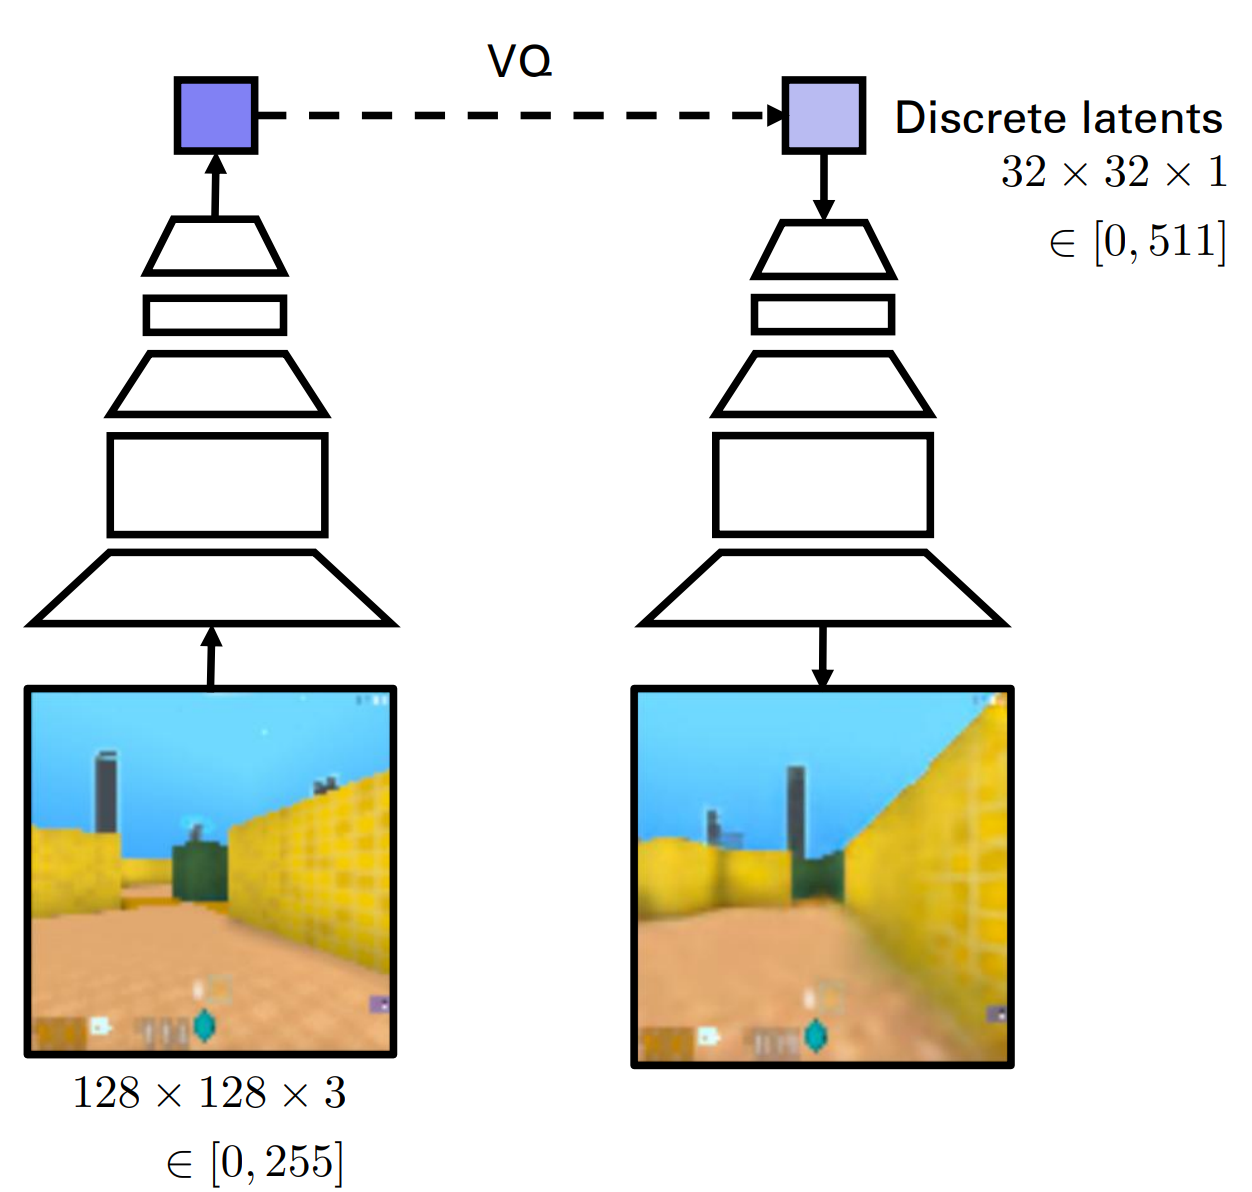
\includegraphics[height=0.8\textheight, width=\textwidth, keepaspectratio]{images/vae/vqvae_b.png}

     {\scriptsize Source: A. van den Oord, ``Neural Discrete Representation Learning,'' SANE 2017 talk slides (DeepMind).}
     \end{center}
\end{column}
\end{columns}
\end{frame}

\begin{frame}[allowframebreaks]{VQ-VAE ImageNet Reconstruction}
\begin{figure}
        \centering
        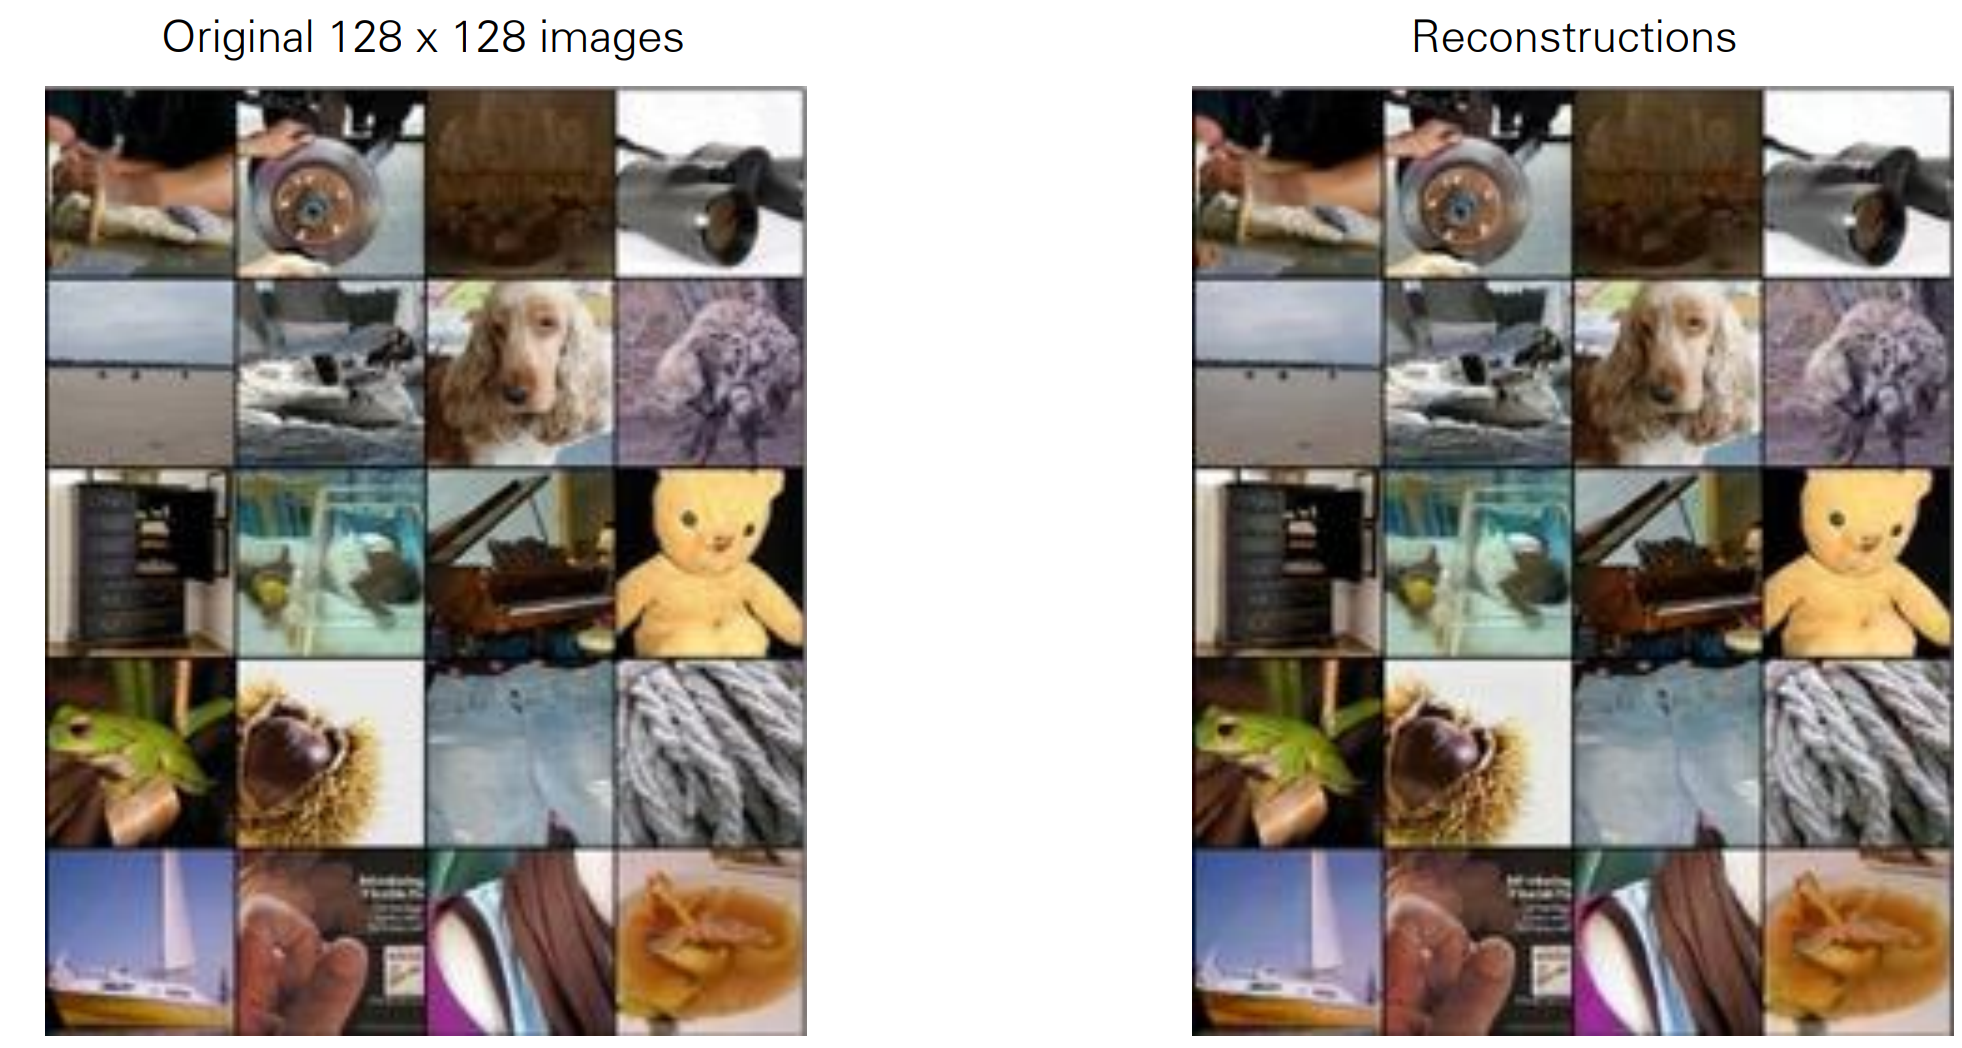
\includegraphics[height=0.8\textheight, width=\textwidth, keepaspectratio]{images/vae/vq_vae_reconstructions.png}
        \caption*{\scriptsize Source: A. van den Oord, ``Neural Discrete Representation Learning,'' SANE 2017 talk slides (DeepMind).}
\end{figure}
\end{frame}

\begin{frame}[allowframebreaks]{VQ-VAE Sampling}
\begin{figure}
        \centering
        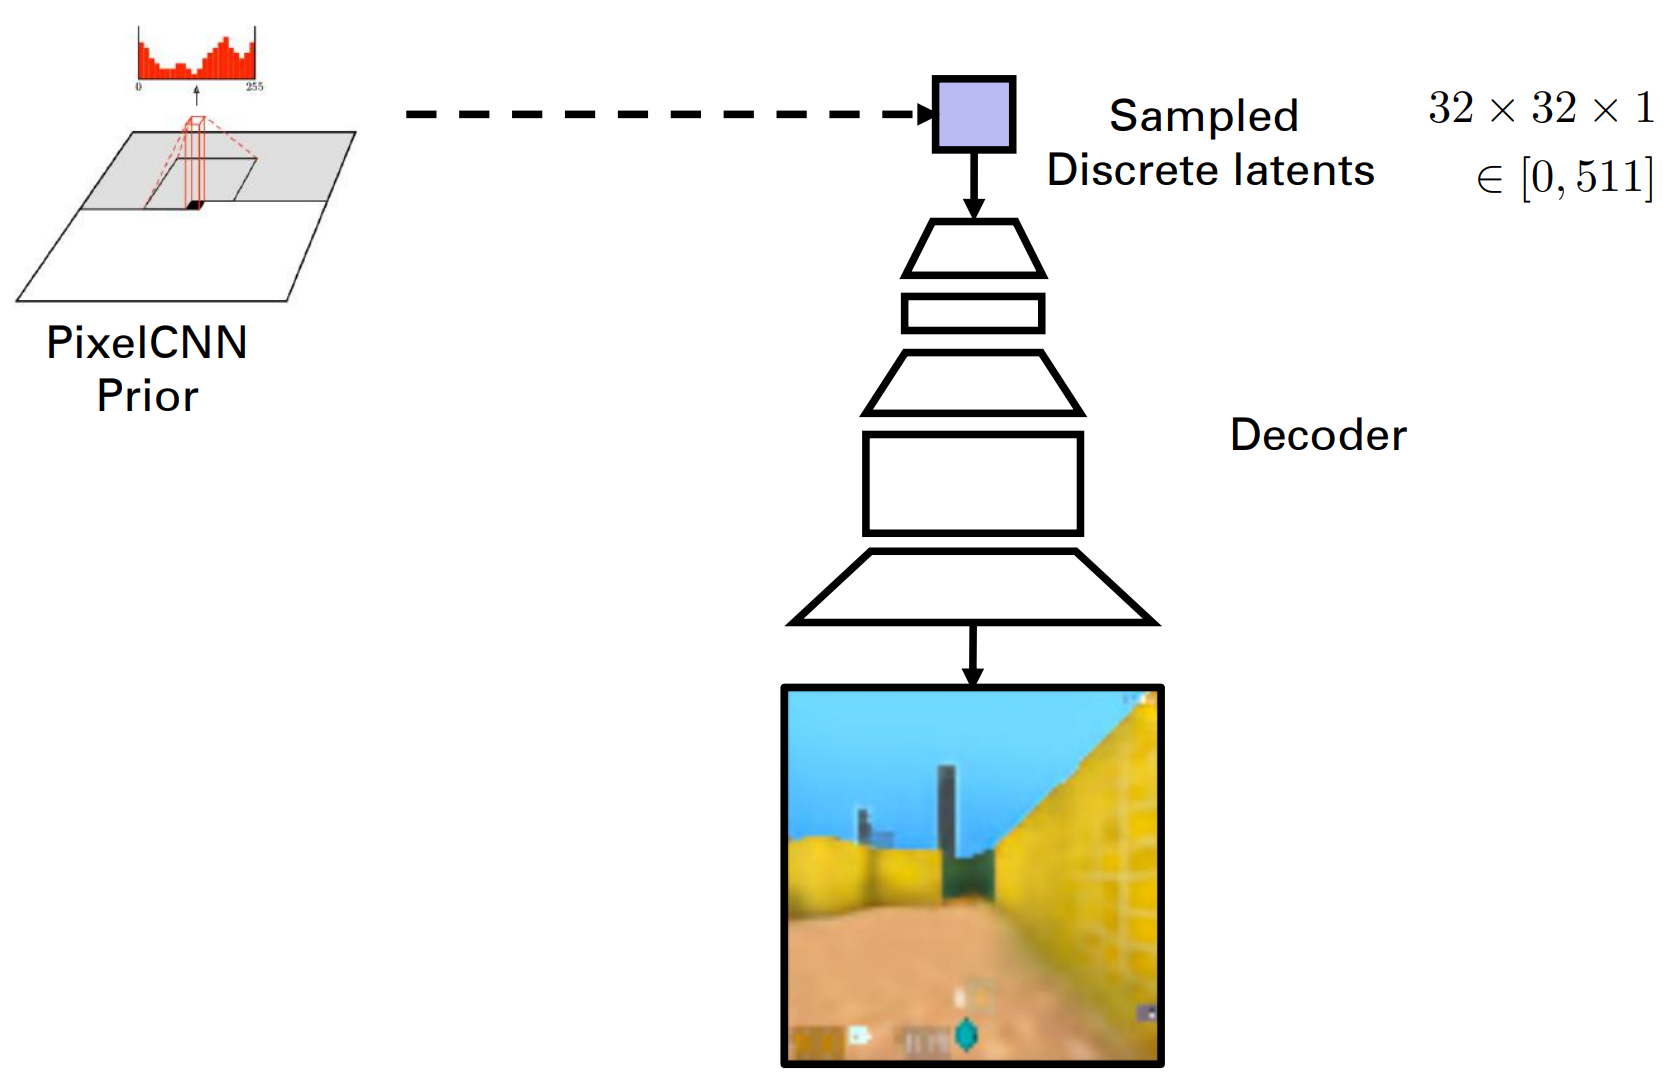
\includegraphics[height=0.8\textheight, width=\textwidth, keepaspectratio]{images/vae/vq_vae_sampling.png}
        \caption*{\scriptsize Source: A. van den Oord, ``Neural Discrete Representation Learning,'' SANE 2017 talk slides (DeepMind).}
\end{figure}
\end{frame}

\begin{frame}[allowframebreaks]{VQ-VAE ImageNet Samples}
\begin{figure}
        \centering
        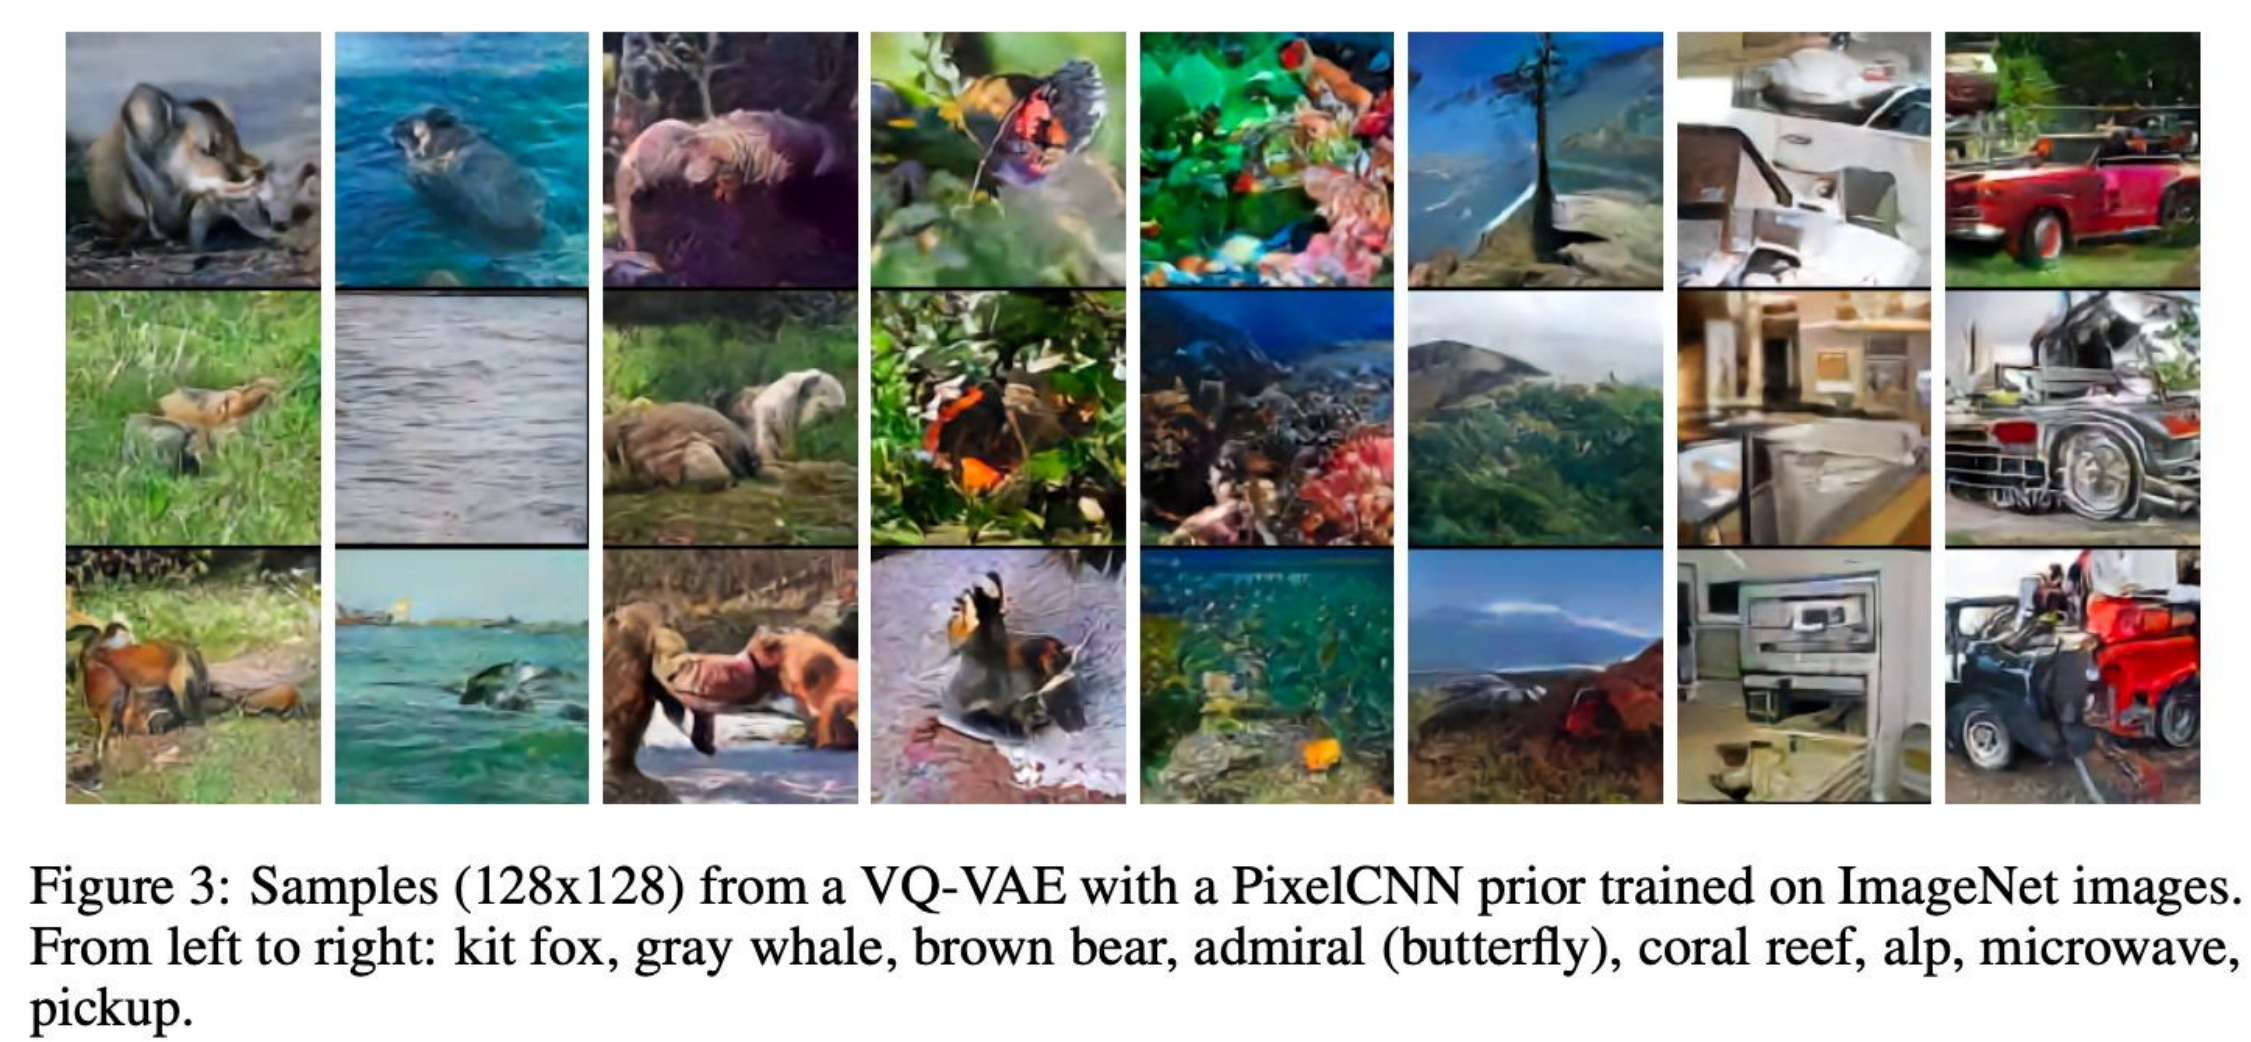
\includegraphics[height=0.8\textheight, width=\textwidth, keepaspectratio]{images/vae/vq_vae_samples.png}
        \caption*{\scriptsize Source: van den Oord, Vinyals \& Kavukcuoglu, ``Neural Discrete Representation Learning,'' NeurIPS 2017, Fig.~3.}
\end{figure}
\end{frame}


\begin{frame}[allowframebreaks]{VQ-VAE Voice Style Transfer}
\begin{figure}
        \centering
        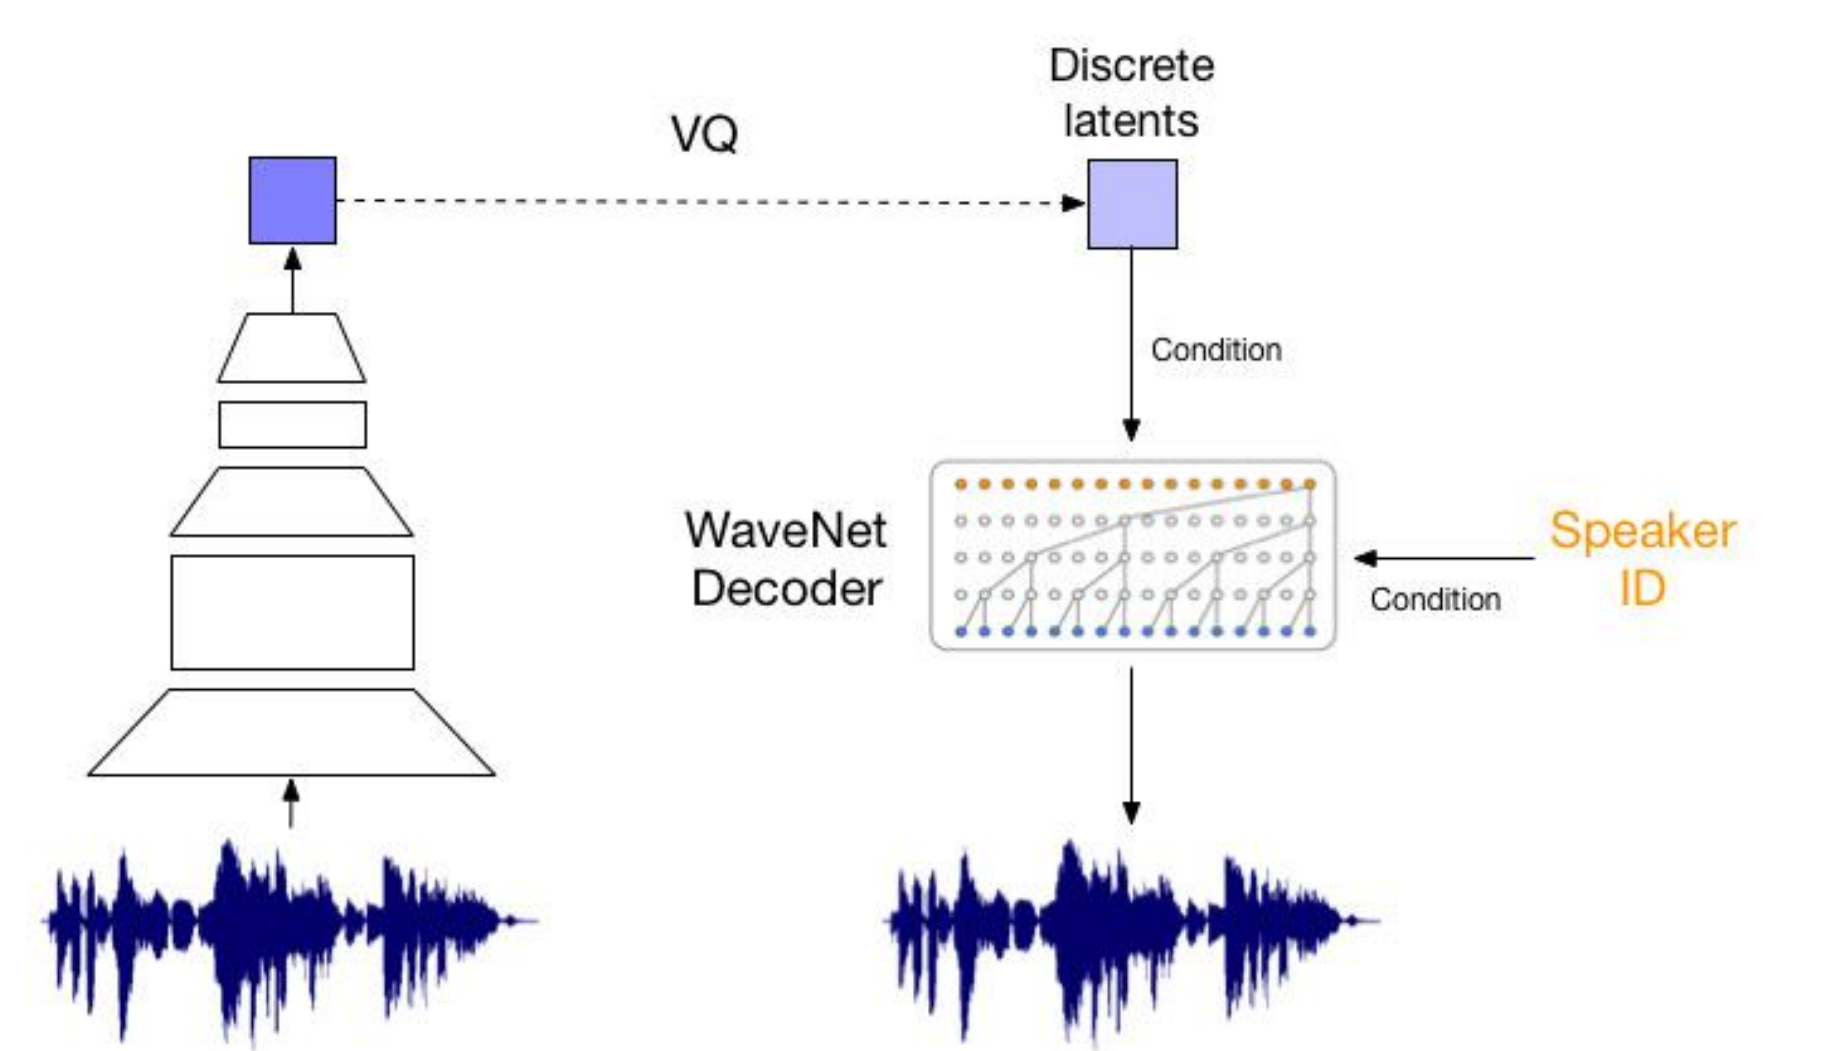
\includegraphics[height=0.8\textheight, width=\textwidth, keepaspectratio]{images/vae/vq_vae_voice.png}
        \caption*{\scriptsize Source: A. van den Oord, ``Neural Discrete Representation Learning,'' SANE 2017 talk slides (DeepMind).}
\end{figure}
\end{frame}

\begin{frame}{VQ-VAE 2}
    \begin{columns}
\begin{column}{0.3\textwidth}
   \begin{itemize}
       \item The input $256 \times 256$ image is compressed to quantized latent maps of size $64 \times 64$ and $32 \times 32$
       \item The decoder reconstructs the image from the two latent maps.
   \end{itemize}
\end{column}
\begin{column}{0.7\textwidth}
    \begin{center}
     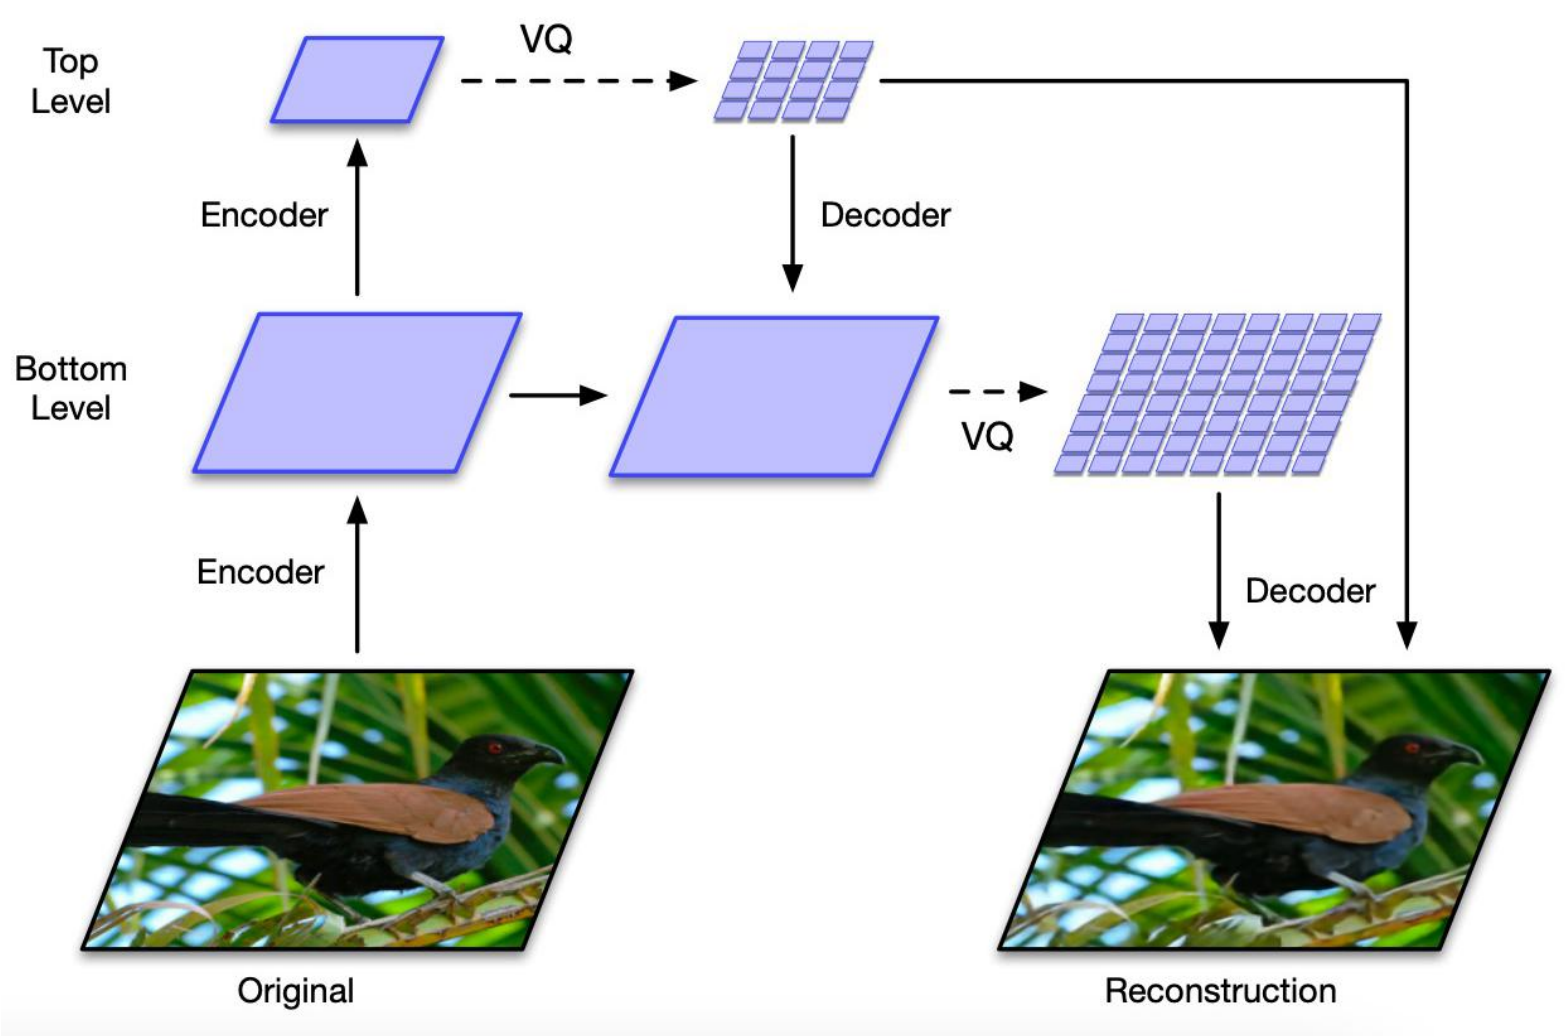
\includegraphics[height=0.8\textheight, width=\textwidth, keepaspectratio]{images/vae/vqvae2.png}

     {\scriptsize Source: Razavi, van den Oord \& Vinyals, ``Generating Diverse High-Fidelity Images with VQ-VAE-2,'' NeurIPS 2019, Fig.~2a.}
     \end{center}
\end{column}
\end{columns}
\end{frame}

\begin{frame}[allowframebreaks]{VQ-VAE-2 Sampling}
\begin{figure}
        \centering
        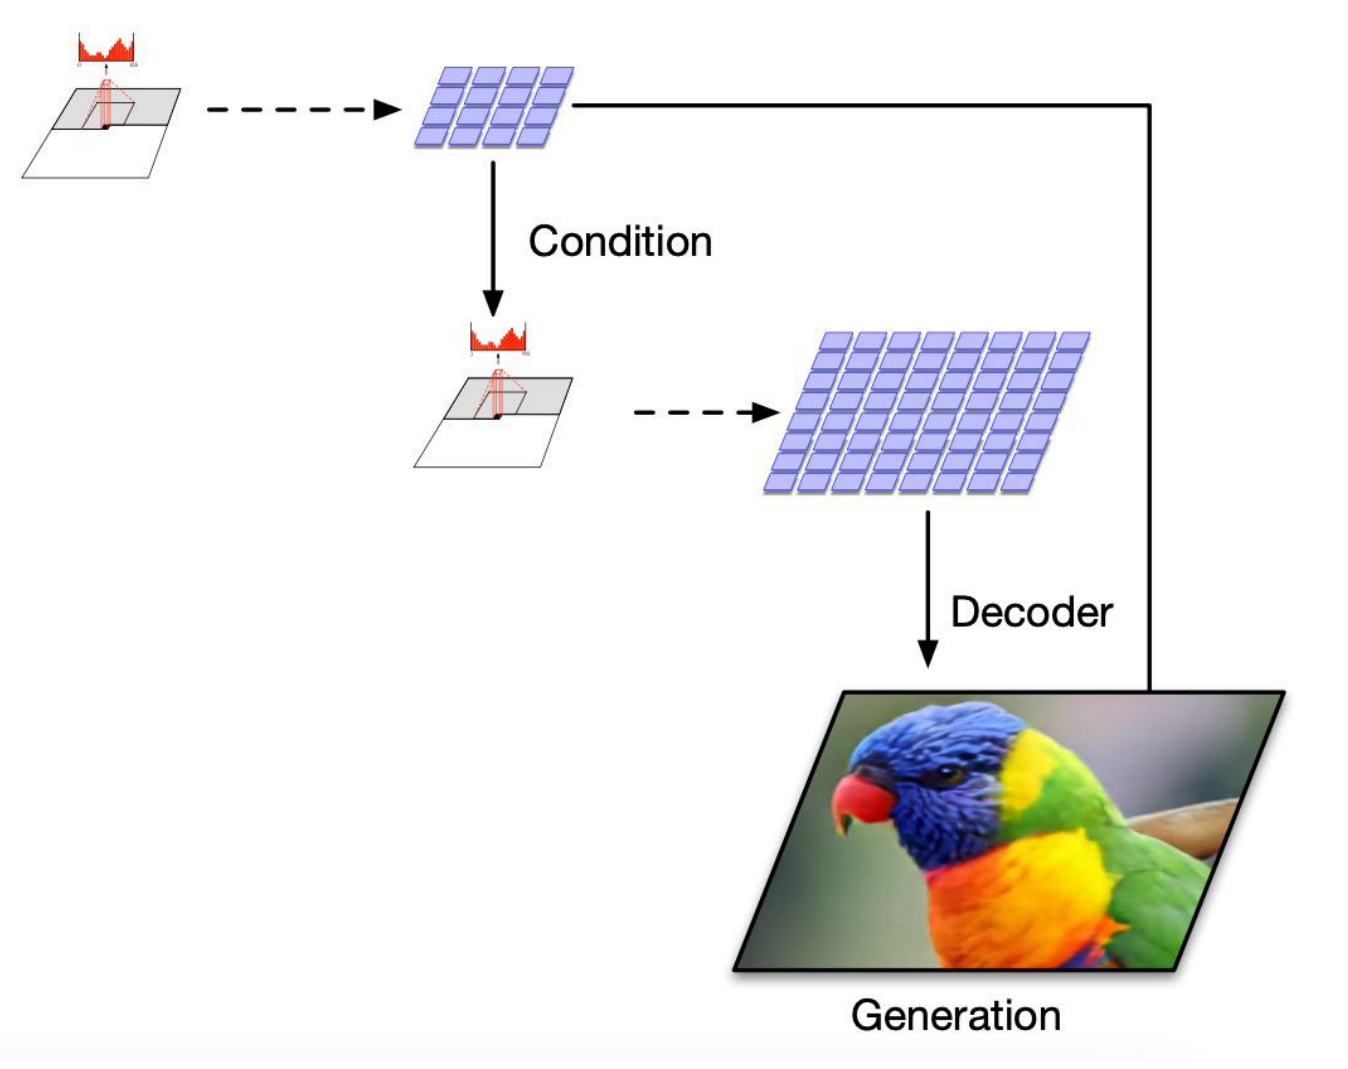
\includegraphics[height=0.8\textheight, width=\textwidth, keepaspectratio]{images/vae/vqvae2_sampling.png}
        \caption*{\scriptsize Source: Razavi, van den Oord \& Vinyals, ``Generating Diverse High-Fidelity Images with VQ-VAE-2,'' NeurIPS 2019, Fig.~2b.}
\end{figure}
\end{frame}

\begin{frame}[allowframebreaks]{VQ-VAE-2 ImageNet Samples}
\begin{figure}
        \centering
        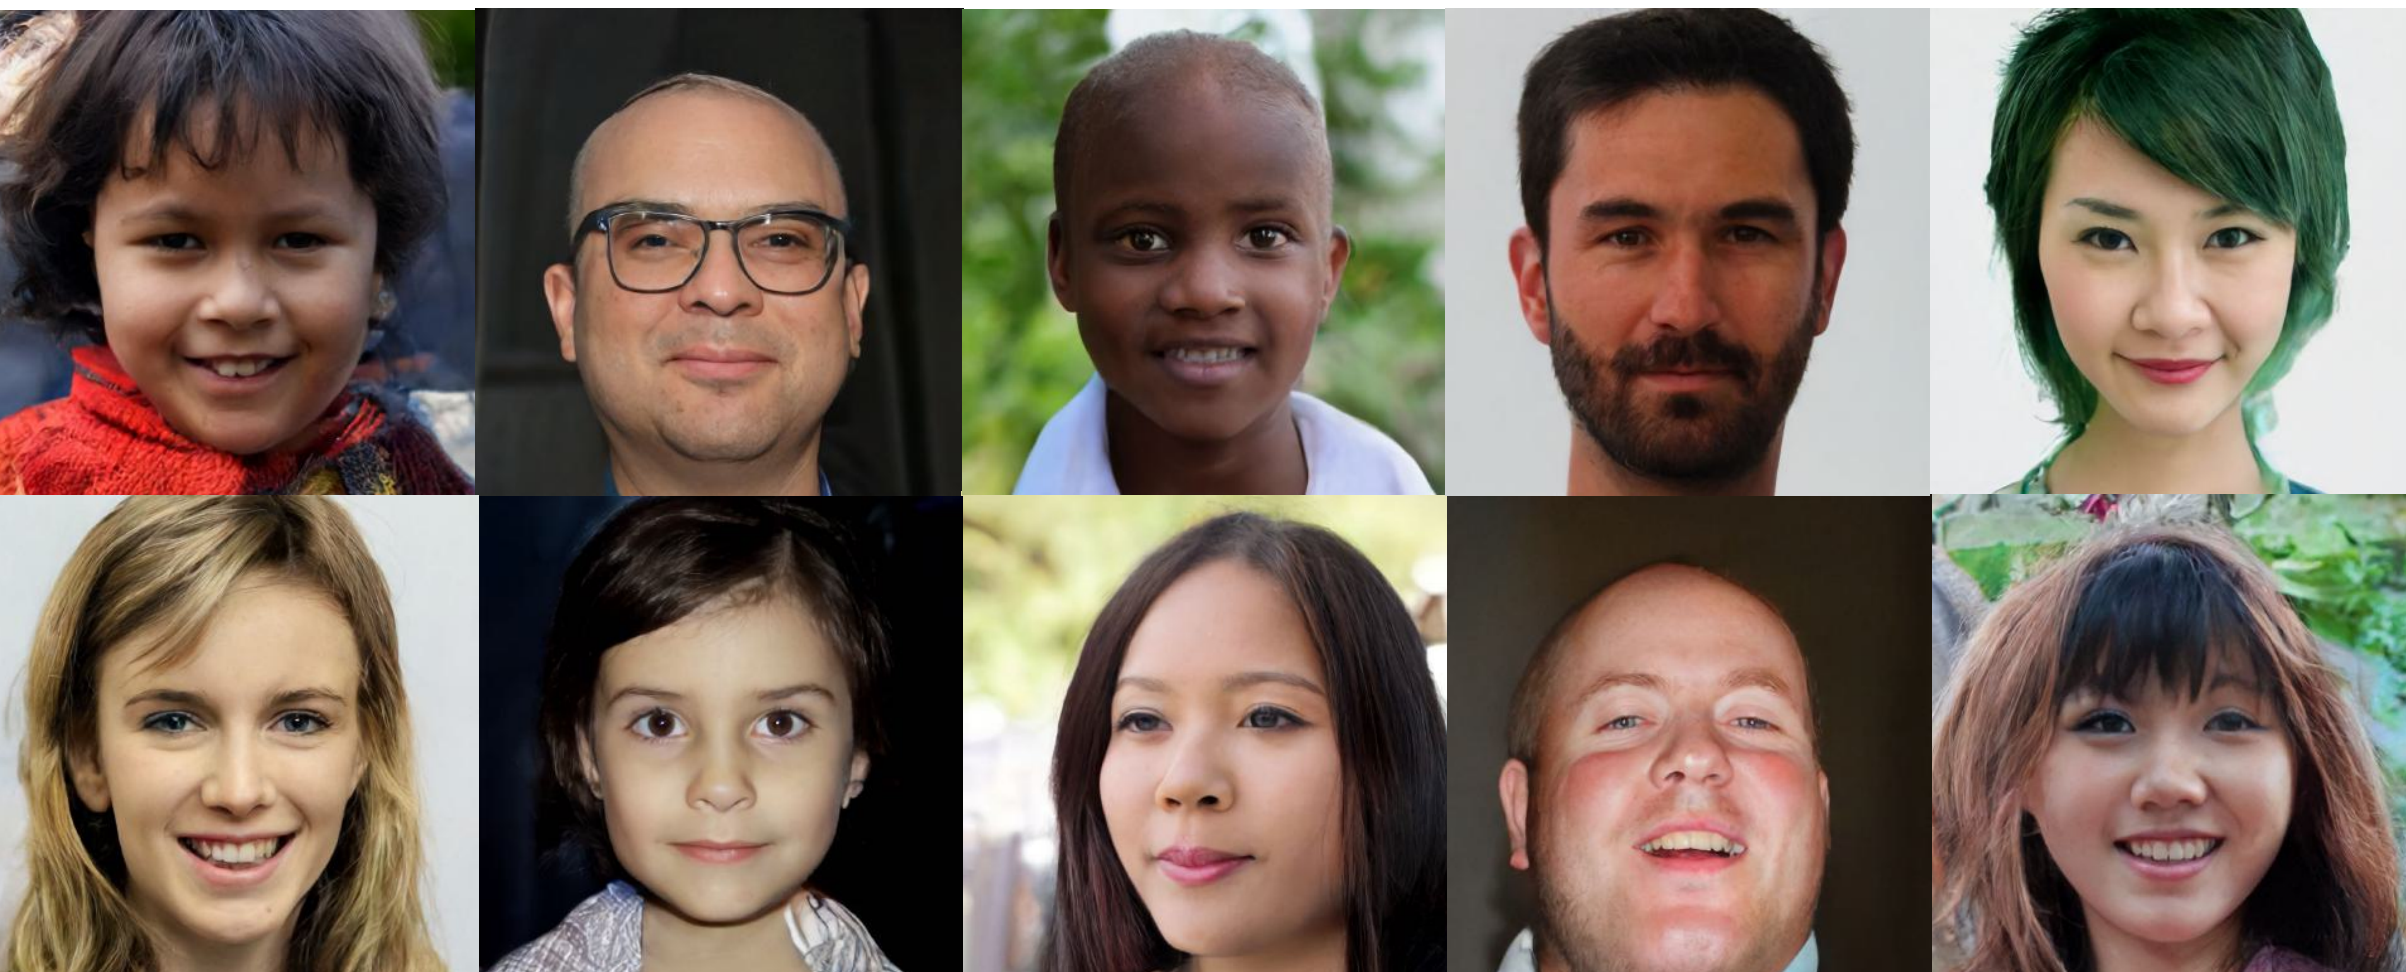
\includegraphics[height=0.8\textheight, width=\textwidth, keepaspectratio]{images/vae/vqvae2_samples.png}
        \caption*{\scriptsize Samples from the three-level hierarchical model trained on FFHQ $1024 \times 1024$. Source: Razavi, van den Oord \& Vinyals, ``Generating Diverse High-Fidelity Images with VQ-VAE-2,'' NeurIPS 2019, Fig.~6.}
\end{figure}
\end{frame}